

\documentclass[runningheads,a4paper,10pt]{etc/llncs}
\usepackage{amssymb}
\usepackage{graphicx}
\usepackage{hyperref}
\usepackage{booktabs}
\usepackage{url}
\usepackage{float}
\usepackage{chngpage}
\usepackage{listings}
\usepackage{apacite}
\usepackage[backend=biber,style=authoryear,sorting=nty]{biblatex}

\usepackage[utf8]{inputenc}
\usepackage[spanish,activeacute]{babel}

\usepackage{longtable}
\usepackage{makecell}


\let\stdsection\section
\renewcommand\section{\newpage\stdsection}
\addbibresource{citations.bib}

\urldef{\mailsa}\path|federico.scenna@gmail.com|    
\newcommand{\keywords}[1]{\par\addvspace\baselineskip
\noindent\keywordname\enspace\ignorespaces#1}

\authorrunning{Lic. Federico Scenna}% Part of LEFT running header
\titlerunning{Análisis de grafos del mercado de criptomonedas}% Part of RIGHT running header

\mainmatter  % start of an individual contribution

% first the title is needed
\title{Análisis de grafos del mercado de criptomonedas}

\author{Lic. Federico Scenna\\ [1cm] {\small Tutor: Dr. Ricardo Maronna}}


\institute{ Maestría en Exploración de Datos y Descubrimiento del Conocimiento \\
Facultad de Ciencias Exactas y Naturales\\ Universidad de Buenos Aires\\
\mailsa
}
\setcounter{tocdepth}{3}


\begin{document}
\let\oldaddcontentsline\addcontentsline
\def\addcontentsline#1#2#3{}
\maketitle
\def\addcontentsline#1#2#3{\oldaddcontentsline{#1}{#2}{#3}}

\newpage

\paragraph{Resumen} En este trabajo se analizan series diarias de precios de distintas criptomonedas entre Agosto del año 2020 y Abril de 2021. A partir de correlaciones
de retornos diarios se visualizaron las relaciones entre los distintos activos. Se
identificaron mayoritariamente altas correlaciones entre los movimientos de pre-
cios y, durante el periodo analizado, el activo Cardano (ADA) como el activo de
referencia del mercado.

\paragraph{Palabras clave} Análisis de grafos, mercados financieros, criptomonedas, blockchain

\tableofcontents

\newpage
\section{Introducción}

El mercado de los criptoactivos atraen atención tanto por los medios, los inversores y los organismos regulatorios. Además de la posibilidad de funcionar como dinero digital, existe una variedad de casos de uso potenciales en otras industrias aparte de la financiera. Los estudios académicos que existen sobre este fenómeno podrían considerarse insuficientes en comparación con el peso que tiene en el discurso público. 

Existen antecedentes de aplicaciones de grafos para analizar dinámicas dentro del conjunto de las finanzas tradicionales. En el trabajo de \cite{towards} se aplica análsis de grafos para estudiar la integracion global y la estabilidad de los mercados bursátiles. A su vez, existen ejemplos de aplicaciones para mercados singulares como \cite{grekmarket}  que han utilizado este tipo de análisis para el mercado bursátil griego. 

En el caso del análisis de grafos para el caso de los criptoactivos, la acotada literatura existente se focaliza en dos aspectos. Por un lado, los criptoactivos se encuentran desarrollados sobre una red distribuida de nodos peer-to-peer que son los que se encargados de validar y registrar las transacciones. En esa dirección, los trabajos de \cite{btc-blockchain} y \cite{btc-btccash} son ejemplos de este foco de estudio. Por el otro lado, los trabajos de  \cite{cryptocurrency_rjc} y \cite{cryptonetwork} aplican el análisis de grafos partiendo de los retornos de los distintos criptoactivos y asi determinar aquellos de referencia en la red. 

Es en este último sentido que el objetivo de este trabajo es analizar los 45 criptoactivos de mayor volumen de mercado del periodo entre 22 de Agosto 2020 y el 24 de Abril 2021. A partir de ciertas metricas obtenidas a partir de los datos recogidos, se realiza un análisis de grafos con una metodología consistente a la literatura mencionada.

\section{Metodología}

\subsection{Materiales y análisis exploratorio}
 Se descargaron
series de precios del sitio coinmarketcap.com a través de la libreria de R crypto \footnote{Disponible en: $https://www.rdocumentation.org/packages/crypto/versions/1.1.3$}. A través de este paquete de R, se descargaron datos diarios de 45 criptoactivos y de cada uno de ellos se encontraron disponibles datos de precio máximo, precio mínimo, precio inicial, volumen y precio de cierre.


A partir de este dataset, se generó una lista para identificar a los activos activos tanto volátiles como estables (estos últimos fueron diseñados para mantener un valor similar al dólar estadounidense). Esta lista resultó de utilidad para poder generar visualizaciones y analizar los grafos.
Tanto los datos como el código de este trabajo se encuentran disponibles un repositorio de Github\footnote{$https://github.com/FedeScenna/Crypto_NetworkAnalysis$}.

Las figuras \ref{fig:stablecoins} y \ref{fig:volatile} muestran el precio de cierre de los activos volátiles y estables respectivamente.  En el caso del comportamiento de los activos volátiles es llamativo el comportamiento del activo YFI (de Yearn Finance, un proyecto de finanzas descentralizadas). Durante el periodo que se toma de análisis para este trabajo este activo alcanzó excepcionalmente valores similares en tendencia al Bitcoin.


\begin{figure}[htp]
    \centering
    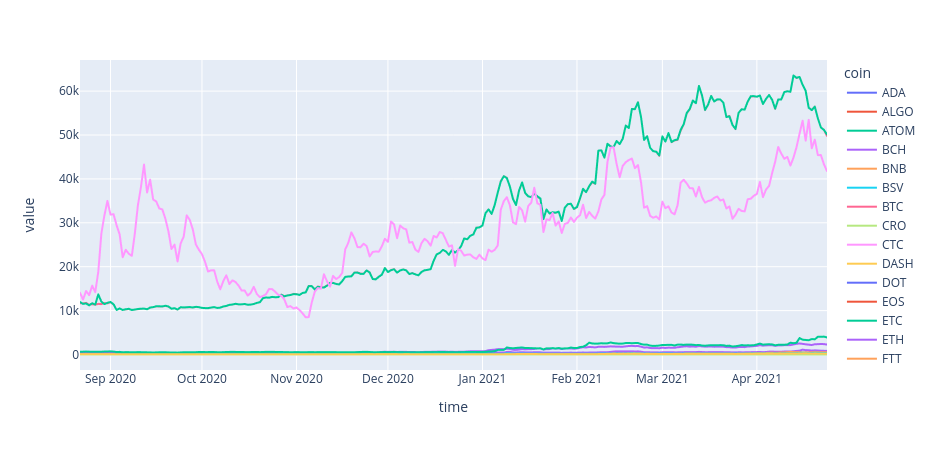
\includegraphics[scale=0.3]{images/volatilecoins_lineplot.png}
    \caption{Precios de monedas volátiles}
    \label{fig:volatile}
\end{figure}

\begin{figure}[htp]
    \centering
    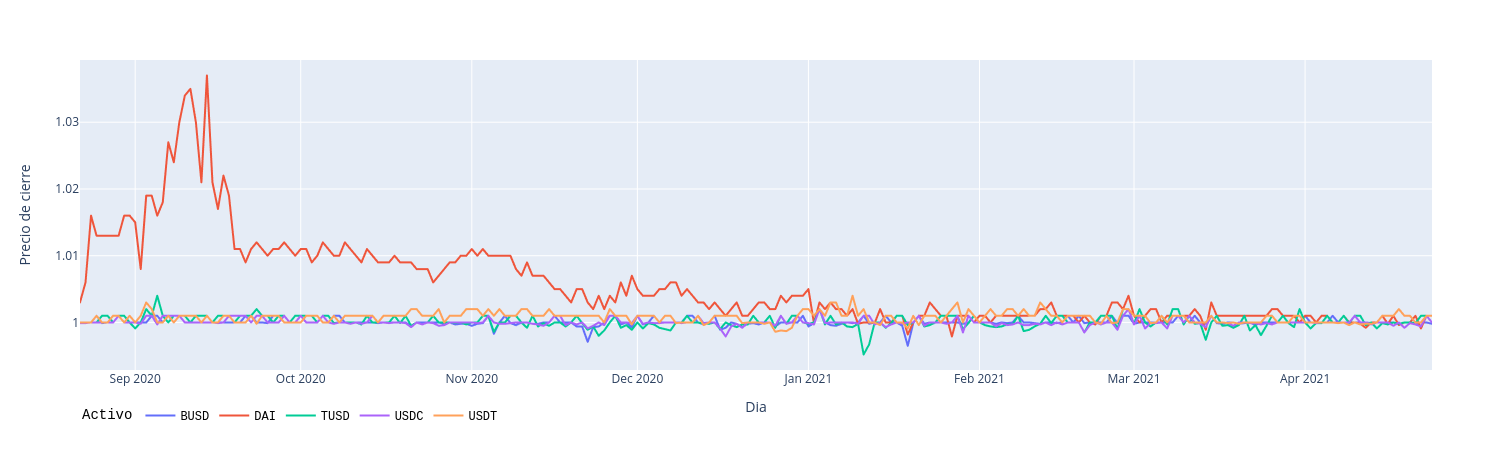
\includegraphics[scale=0.3]{images/stablecoins_lineplot.png}
    \caption{Precios de monedas estables}
    \label{fig:stablecoins}
\end{figure}


\subsection{Transformacion de datos}
Previamente a la construcción del grafo, era necesario establecer alguna
métrica para desestacionalizar la serie de precios de los activos para evitar correlaciones espurias. Uno de los métodos más frecuentes que propone la literatura \cite{cryptonetwork} es la tasa de retorno logarı́tmica:
\begin{math} log(p_t) -log(p_t-1) \end{math}

Se decidió, a modo de mantener la claridad en el análisis y por las cualidades
propias del este tipo de mercado, computar retornos diarios de cada uno de los
activos. La distribución del mismo para cada uno de los activos se puede visualizar en la figura \ref{fig:box_returns}. Lo más resaltable de este gráfico es la dispersión del retorno de algunos activos (como HEX o HEDG) que no forman parte de las carteras mas tradicionales de inversiones.
La tabla \ref{tab:desc_stats} muestra un resumen estadistico de los retornos para los distintos activos. A partir de esta información, es notorio que los rendimientos promedios son bajos o en algunos casos nulos. Sin embargo, debido a la dispersión de rendimientos, resultan llamativos dos casos: CTC que alcanzó un alza diaria de 384\% y HEX con una baja de -100.4\%.

\begin{longtable}{lrrrrrr}\n
\toprule
\n Coin &  Maximum &  Minimum &     Mean &  Standard Deviation &  Kurtosis &     Skew \\\\\n
\midrule\n  ADA &  0.28690 & -0.19863 &  0.00901 &             0.06734 &   2.15015 &  0.59927 \\\\\n ALGO &  0.32757 & -0.28160 &  0.00306 &             0.07064 &   2.22789 &  0.22113 \\\\\n ATOM &  0.28779 & -0.28904 &  0.00510 &             0.07274 &   2.22941 &  0.35016 \\\\\n  BCH &  0.27502 & -0.22931 &  0.00432 &             0.06084 &   3.89279 &  0.00835 \\\\\n  BNB &  0.53325 & -0.27032 &  0.01279 &             0.07382 &  11.36871 &  1.68906 \\\\\n  BSV &  0.45853 & -0.27835 &  0.00089 &             0.06362 &  12.19433 &  1.08539 \\\\\n  BTC &  0.17791 & -0.14075 &  0.00595 &             0.03759 &   2.63961 &  0.16353 \\\\\n BUSD &  0.00341 & -0.00301 & -0.00000 &             0.00074 &   3.66824 & -0.13204 \\\\\n  CRO &  0.48397 & -0.36777 & -0.00006 &             0.06526 &  15.97548 &  0.91327 \\\\\n  CTC &  3.84155 & -0.13572 &  0.02473 &             0.25241 & 215.73318 & 14.25435 \\\\\n  DAI &  0.01555 & -0.01555 & -0.00002 &             0.00245 &  15.89812 &  0.44309 \\\\\n DASH &  0.45446 & -0.22069 &  0.00437 &             0.06859 &   8.80728 &  1.31567 \\\\\n  DOT &  0.46012 & -0.21479 &  0.00976 &             0.07638 &   6.52699 &  1.60595 \\\\\n  EOS &  0.15550 & -0.22694 &  0.00203 &             0.05931 &   1.96096 & -0.15718 \\\\\n  ETC &  0.36493 & -0.20059 &  0.00633 &             0.07117 &   5.20492 &  1.06322 \\\\\n  ETH &  0.23348 & -0.21475 &  0.00717 &             0.05110 &   2.54604 & -0.24656 \\\\\n  FTT &  0.27724 & -0.17198 &  0.01075 &             0.05263 &   3.75757 &  0.58575 \\\\\n HEDG &  1.28813 & -0.31939 & -0.00172 &             0.12300 &  54.49864 &  5.81430 \\\\\n  HEX &  1.03805 & -1.00402 &  0.00698 &             0.22810 &   5.81884 & -0.08437 \\\\\n   HT &  0.48709 & -0.22037 &  0.00548 &             0.06203 &  16.34554 &  1.83903 \\\\\n  LEO &  0.12413 & -0.10863 &  0.00238 &             0.02068 &  13.57275 &  0.55425 \\\\\n LINK &  0.25630 & -0.20421 &  0.00365 &             0.06798 &   0.85816 &  0.13176 \\\\\n  LTC &  0.16930 & -0.19972 &  0.00561 &             0.05637 &   1.32901 & -0.12723 \\\\\n MIOTA &  0.28113 & -0.20185 &  0.00638 &             0.06541 &   2.37966 &  0.36100 \\\\\n  MKR &  0.43207 & -0.20780 &  0.00757 &             0.06799 &   9.79891 &  1.88809 \\\\\n  NEO &  0.24436 & -0.20666 &  0.00654 &             0.06370 &   1.59984 &  0.14850 \\\\\n  OKB &  0.49342 & -0.23070 &  0.00449 &             0.06981 &  17.67954 &  2.62858 \\\\\n  OMG &  0.23489 & -0.25455 &  0.00007 &             0.07541 &   1.02414 &  0.12268 \\\\\n  ONT &  0.16712 & -0.27832 &  0.00221 &             0.06729 &   1.78862 & -0.62278 \\\\\n  SNX &  0.18588 & -0.24255 &  0.00399 &             0.07609 &   0.17881 &  0.05737 \\\\\n THETA &  0.25949 & -0.20796 &  0.01266 &             0.07194 &   0.98019 &  0.42555 \\\\\n  TRX &  0.34353 & -0.18786 &  0.00597 &             0.06354 &   4.03662 &  0.83670 \\\\\n TUSD &  0.00331 & -0.00461 &  0.00000 &             0.00110 &   1.24297 & -0.23173 \\\\\n  UMA &  0.46812 & -0.42223 &  0.00506 &             0.09986 &   6.44948 &  1.22827 \\\\\n USDC &  0.00250 & -0.00250 &  0.00000 &             0.00071 &   2.06077 &  0.05611 \\\\\n USDT &  0.00299 & -0.00300 &  0.00000 &             0.00086 &   1.05759 & -0.04404 \\\\\n  VET &  0.29010 & -0.25489 &  0.00963 &             0.07888 &   1.30245 &  0.37121 \\\\\n WBTC &  0.18686 & -0.14075 &  0.00596 &             0.04069 &   3.27039 &  0.31365 \\\\\n  XEM &  0.25028 & -0.45924 &  0.00541 &             0.07852 &   5.83846 & -0.51516 \\\\\n  XLM &  0.58520 & -0.24639 &  0.00608 &             0.07915 &  14.10666 &  2.33161 \\\\\n  XMR &  0.22375 & -0.16367 &  0.00536 &             0.05043 &   3.07137 &  0.19233 \\\\\n  XRP &  0.45137 & -0.53823 &  0.00568 &             0.08935 &  10.22325 &  0.37084 \\\\\n  XTZ &  0.19744 & -0.19940 &  0.00128 &             0.05879 &   1.69904 & -0.17453 \\\\\n  YFI &  0.37740 & -0.21103 &  0.00498 &             0.08984 &   1.83518 &  0.78047 \\\\\n  ZEC &  0.20925 & -0.28939 &  0.00428 &             0.06544 &   2.01915 & -0.30462 \\\\\n
\bottomrule
\n
\caption{Estadísticas de resumen del retorno de los criptoactivos}
\label{tab:desc_stats}
\end{longtable}

\begin{figure}[htp]
    \centering
    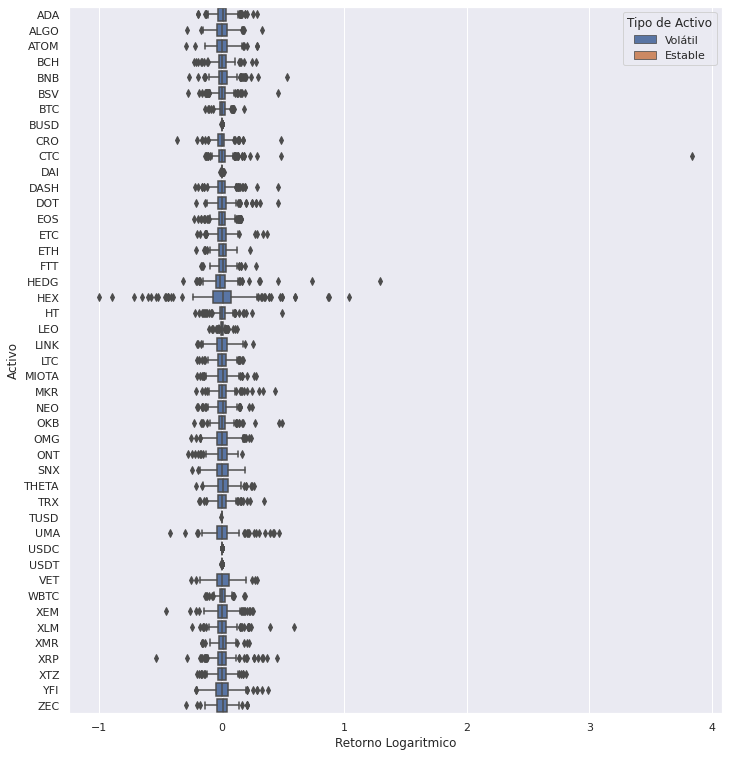
\includegraphics[scale=0.3]{images/box_returns.png}
    \caption{Boxplot de los retornos de los criptoactivos}
    \label{fig:box_returns}
\end{figure}

A partir de esta métrica de retorno, se calculó la matriz a partir de la correlación de Pearson (ver figura \ref{fig:corr_matrix}). Adicionalmente, se puede ver la distribución de las correlaciones de esta matriz en la figura \ref{fig:hist_corr}. A partir de estos gráficos, se concluye que las distribución de las correlaciones tienen una forma bimodal.


\begin{figure}[htp]
    \centering
    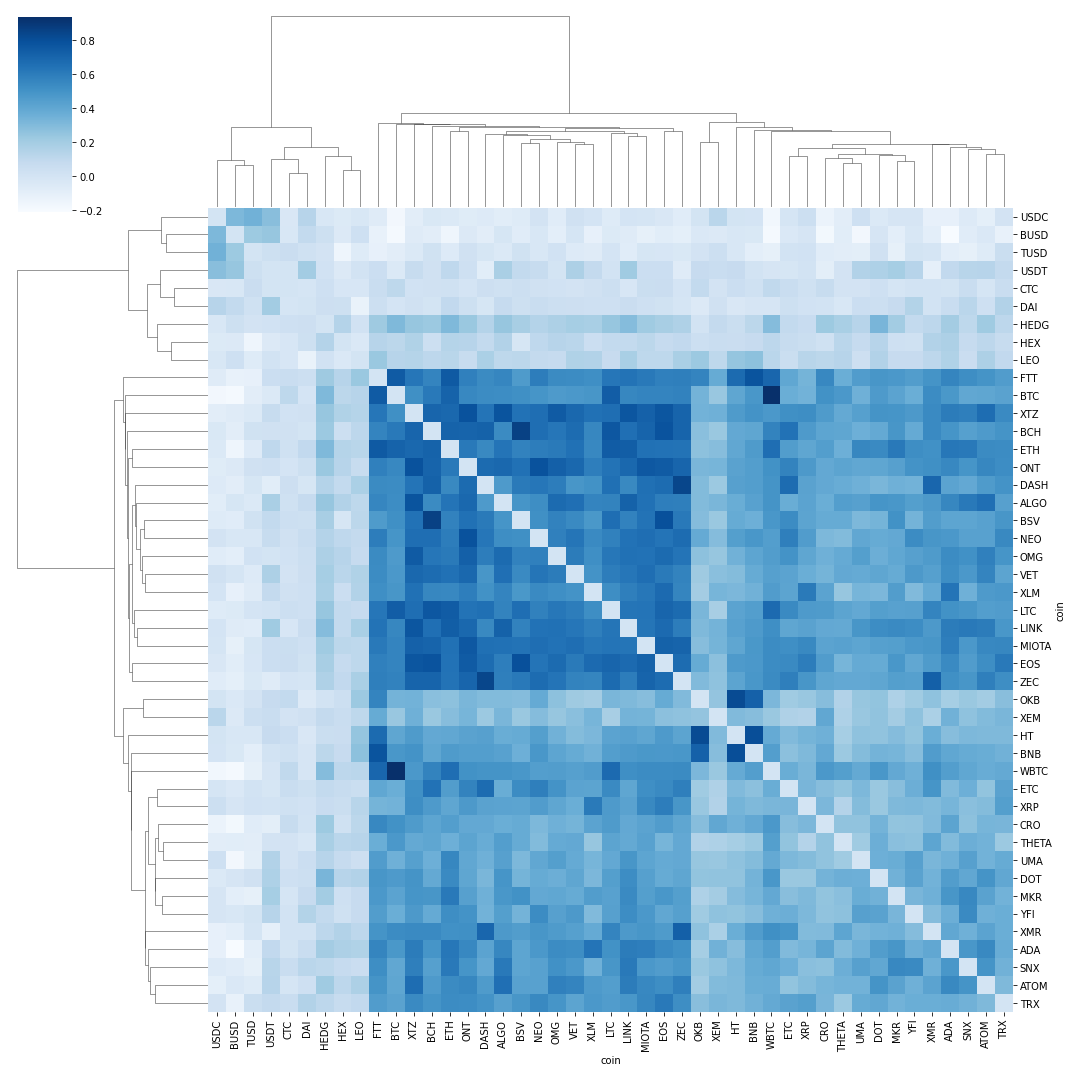
\includegraphics[scale=0.3]{images/corr_matrix.png}
    \caption{Matriz de correlación de los activos}
    \label{fig:corr_matrix}
\end{figure}


\begin{figure}[htp]
    \centering
    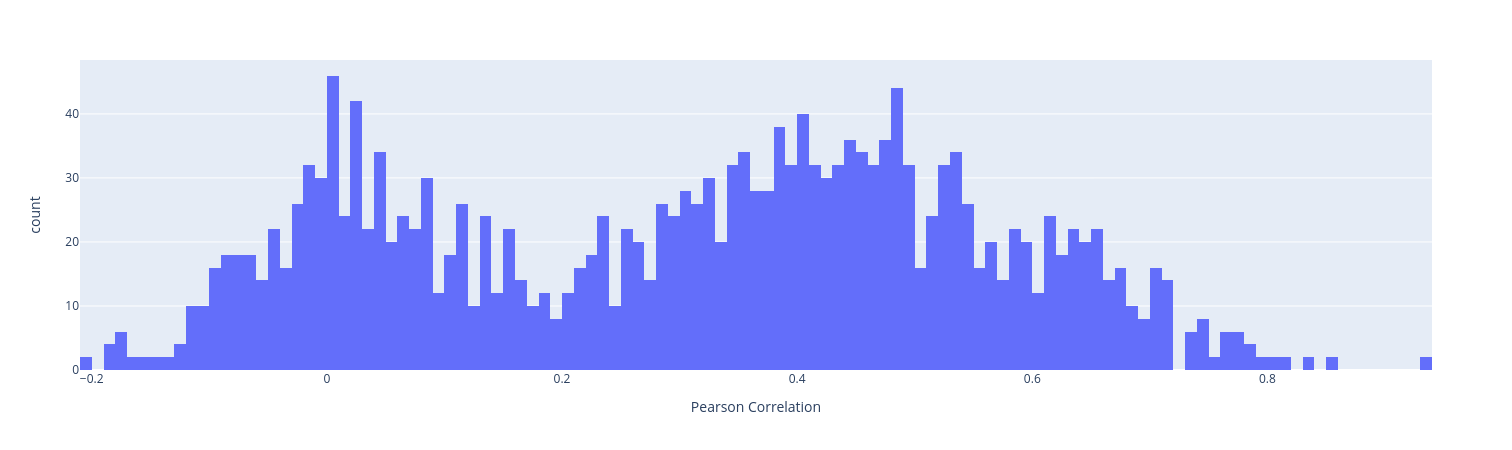
\includegraphics[scale=0.3]{images/correlation_hist.png}
    \caption{Histograma de correlación de los activos}
    \label{fig:hist_corr}
\end{figure}
\section{Resultados}
\subsection{Visualizaciones} 


En la literatura, la metodologı́a usualmente propuesta es la creación de un grafo a partir de una matriz de correlación con un punto de corte determinado.
En base a la distrubición de la correlación y a la centralidad de intermediación (betweenness centrality, ver figura \ref{fig:btw_centrality}) promedio de la red, se tomo como valor de corte las aristas entre activos con una correlación mayor al 20\%.

\begin{figure}[htp]
    \centering
    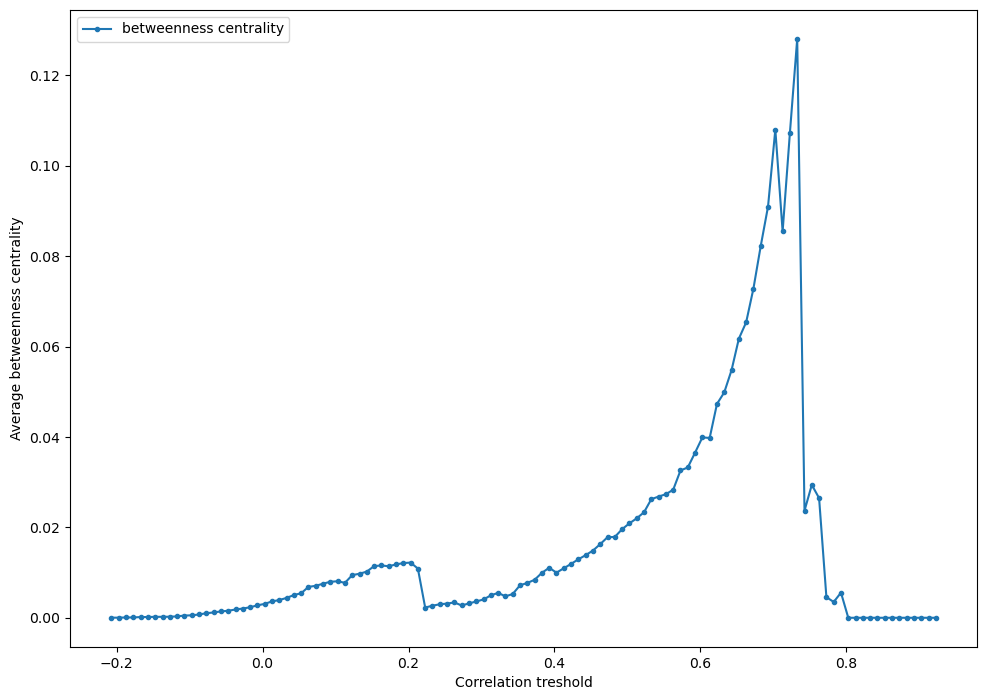
\includegraphics[scale=0.3]{images/betweeness_centrality.png}
    \caption{Ćentralidad de intermediación}
    \label{fig:btw_centrality}
\end{figure}


A partir de este punto de corte y consistente con la literatura, se construyó un Minimum Spanning Tree (MST) que puede visualizarse a continuación en la figura \ref{fig:mst}:

\begin{figure}[htp]
    \centering
    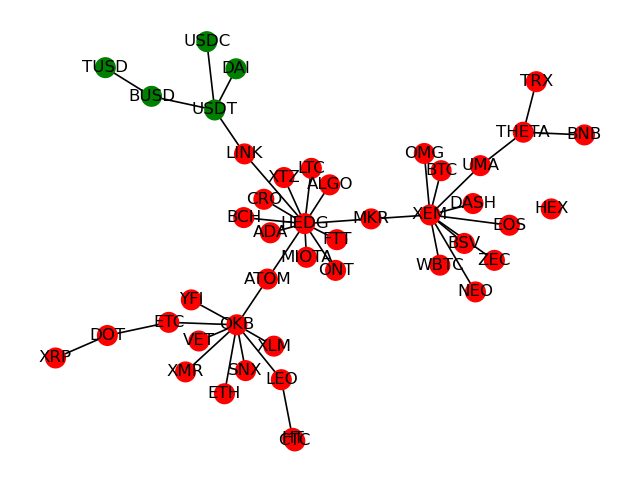
\includegraphics[scale=1]{images/mst.png}
    \caption{MST de los activos}
    \label{fig:mst}
\end{figure}

A partir de esta estructura, se puede visualizar las distancias relativas de los nodos en función de la correlación que tienen entre si. De tal manera, cuan más cerca se encuentren dos nodos mayor es la correlación que existe entre ellos. 

\subsection{Búsqueda de comunidades}

Una herramienta recurrente en el análisis de grafos es la búsqueda de comunidades. Según \cite{networkscience}, se define como comunidad a un grupo de nodos que poseen una probabilidad más alta de conectarse entre sí respecto a otros nodos. Para la búsqueda de comunidades se emplearon dos algoritmos: Louvain y Girvan-Neuman. 

Del resultado de ambos se tomo el algoritmo que arrojaba modularidad más alta. El ganador fue el algoritmo Louvain (figura \ref{fig:community_louvain}) cuya modularidad de 0.68 arrojó mejores resultados que Girvan-Neuman (ver figura \ref{fig:community_gn}). En la imagen siguiente se puede visualizar el resultado de las comunidades encontradas por este algoritmo. El mismo pudo separar adecuadamente los activos estables de los volátiles.


\begin{figure}[htp]
    \centering
    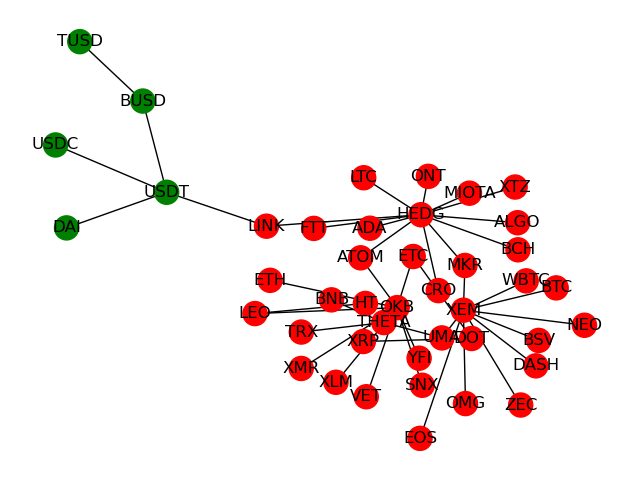
\includegraphics[scale=1]{images/community_louvain.png}
    \caption{Resultado del algoritmo Louvain}
    \label{fig:community_louvain}
\end{figure}

\begin{figure}[htp]
    \centering
    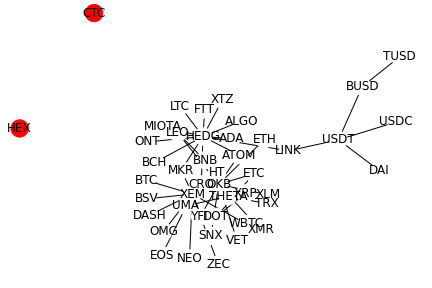
\includegraphics[scale=1]{images/community_gn.png}
    \caption{Resultado del algoritmo Girvan-Neuman}
    \label{fig:community_gn}
\end{figure}

\section{Conclusiones}

En el caso puntual de este trabajo, hay algunas cualidades que deben resaltarse. En primer lugar, se diferencia claramente entre las monedas estables (resaltadas en verde) y las monedas volátiles (en rojo). 

En segundo lugar, observamos que hay dos activos que se encuentran visiblemente desacoplados del resto de los activos del grafo: CTC (Creditcoin) y HEX (Hex.com). El primero es un token de una blockchain destinada a facilitar capital de crédito y trazabilidad de transacciones a fintechs y a proyectos de microfinanzas. El segundo es un proyecto de finanzas descentralizadas destinado a ofrecer alto interés por depósitos a plazo fijo. Sin embargo, han surgido algunas opiniones cuestionando que pueda afianzarse como un proyecto a largo plazo.

En tercer lugar, se puede observar 4 subgrafos de activos que se encuentran conectados entre sí. Lo que es particularmente interesante son los tres subgrafos de monedas volátiles ya que ni ETH ni BTC son los activos de referencia de esos subgrafos. De esta manera, se constituye una discrepancia respecto a la literatura consultada para este trabajo.


\printbibliography %[citations]



\end{document}